\documentclass{beamer}

% Encoding & language
\usepackage[T1]{fontenc}
\usepackage[utf8]{inputenc}
\usepackage[english]{babel}
\usepackage{transparent}

% Bibliography
\usepackage[numbers]{natbib}
\bibliographystyle{ieeetr}

% Figures, tables, colors
\usepackage{graphicx}
\usepackage{subcaption}
\usepackage{tabularx}
\usepackage{booktabs}
\usepackage{multirow}
\usepackage{makecell}
\usepackage[table, svgnames]{xcolor}

\usepackage{caption}
\captionsetup[table]{justification=centering}

% Beamer
\setbeamerfont{framesubtitle}{size=\normalsize}

% Misc
\usepackage{amsmath}
\usepackage{amssymb}
\usepackage{hyperref}
\usepackage{tikz}
\usetikzlibrary{arrows.meta, positioning}
\DeclareMathOperator{\jinc}{jinc}

% Transparent, Checkmark
\usepackage{transparent}
\newcommand{\dimtxt}[1]{{\transparent{0.25}#1}} % 0.25-0.45
\usepackage{pifont}
\newcommand{\cmark}{\ding{51}}
\newcommand{\xmark}{\ding{55}}

\mode<presentation>{
  \usetheme{Madrid}
  \usecolortheme{default}
  \setbeamertemplate{caption}[numbered]
}

\title[Solar Radio Interferometer Simulation]{%
  {\Large\bfseries End-to-End Simulation of a Four-Element UHF Radio\\
  Interferometer for Solar Radio Observation at 610~MHz}%
}

\subtitle{Graduation Thesis Defense}

\author[N. B. Quan]
{Nguyen Ba Quan (20224350) \\ Supervisor: Assoc.\ Prof.\ Dr.\ Ha Duyen Trung}

\institute[SEEE--HUST]
{
School of Electrical and Electronic Engineering \\
Hanoi University of Science and Technology
}

\date{\today}

\setbeamertemplate{bibliography item}{\insertbiblabel}

\begin{document}

% ============================================================
% Title
\begin{frame}
  \titlepage
\end{frame}

\AtBeginSection[]
{
  \begin{frame}
    \frametitle{Outline}
    \tableofcontents[currentsection]
  \end{frame}
}

% ============================================================
\section{Motivation}

\begin{frame}{Space Weather: Why It Matters}
\begin{columns}[c]
\column{.52\textwidth}
\begin{itemize}
  \item Solar eruptive activity (flares, CMEs) drives \textbf{space weather} that
  disturbs satellites, GNSS links, and power grids.
  \item Solar Cycle 25 reached its maximum phase in Oct.\ 2024~\cite{nasa_noaa_solarmax2024}.
  \item \textbf{2022 Starlink incident}: a geomagnetic storm dragged \textbf{38 of
  49} newly launched satellites back into the atmosphere within days~\cite{berger2023starlink}.
  \item \textbf{GNSS impact}: bursts perturb the ionosphere's free electrons,
  inducing \textbf{positional error} in GPS/Galileo receivers~\cite{floressoriano2024gnss}.
\end{itemize}
\column{.46\textwidth}
\centering
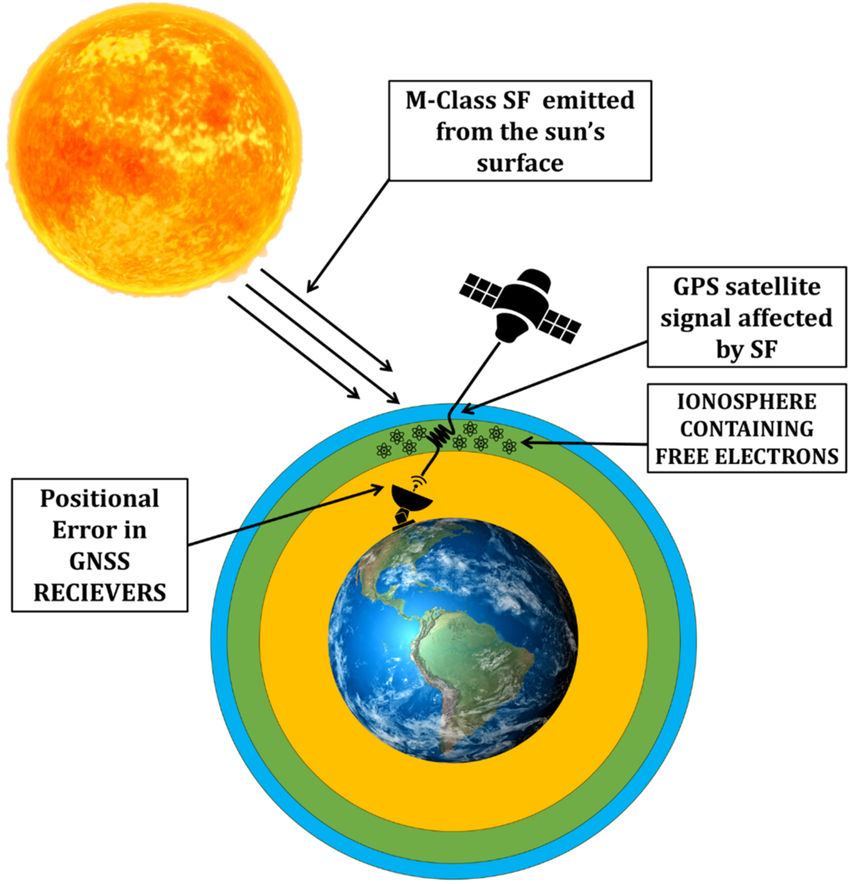
\includegraphics[height=0.52\textheight]{figs/fig_gnss_ionosphere.png}
\vspace{2pt}
\small Solar burst $\to$ ionospheric disturbance $\to$ GNSS positional error.
\end{columns}
\end{frame}

\begin{frame}{Why Radio Interferometry?}
\begin{itemize}
  \item Solar radio bursts are an \textbf{early, ground-observable} signature of eruptive activity.
  \item A single dish resolving the $32'$ solar disk would need to be
  \textbf{tens of metres} across --- expensive, hard to build for a university lab.
  \item \textbf{Radio interferometry}: combine several \emph{small} antennas;
  resolution then depends on the \emph{baseline}, not on a single dish diameter.
\end{itemize}
\vspace{0.4em}
\begin{block}{Precedent: DLITE}
A four-element, field-deployable, low-cost interferometer
(30--40~MHz, LWA-style dipoles, $\approx$\$1{,}200/antenna) that has
already detected Type~II/III solar radio bursts~\cite{carson2022dlite,lwa_pricing}.
\end{block}
\centering
\textbf{$\Rightarrow$ Low-cost, distributed arrays are a realistic path to solar radio monitoring.}
\end{frame}

\begin{frame}{Why 610~MHz?}
\begin{itemize}
  \item Not where the strongest bursts occur (those favour tens of MHz), but a
  \textbf{practical} UHF choice:
  \begin{enumerate}
    \item Learmonth/SWS already publishes \textbf{free, continuous, real} 610~MHz
    solar flux data.
    \item UHF Yagi-Uda antennas at this band are \textbf{cheap and easy to build}.
    \item Wavelength $\approx 0.49$~m $\Rightarrow$ a baseline of only a few metres
    already produces a clear, measurable fringe.
  \end{enumerate}
\end{itemize}
\end{frame}

\begin{frame}{Prior Work: Field Deployment at Xuan Mai}
\begin{columns}[c]
\column{.5\textwidth}
\begin{itemize}
  \item Two-element Yagi-Uda interferometer deployed at Xuan Mai, Hanoi.
  \item Result: only an \textbf{ambiguous daily trend}, not a clean interferometric detection.
\end{itemize}
\textbf{Root causes identified:}
\begin{itemize}
  \item Phase-incoherent receiver oscillators
  \item Cable insertion loss
  \item Strong local RFI
  \item Noise floor close to quiet-Sun signal level
\end{itemize}
\column{.5\textwidth}
\centering
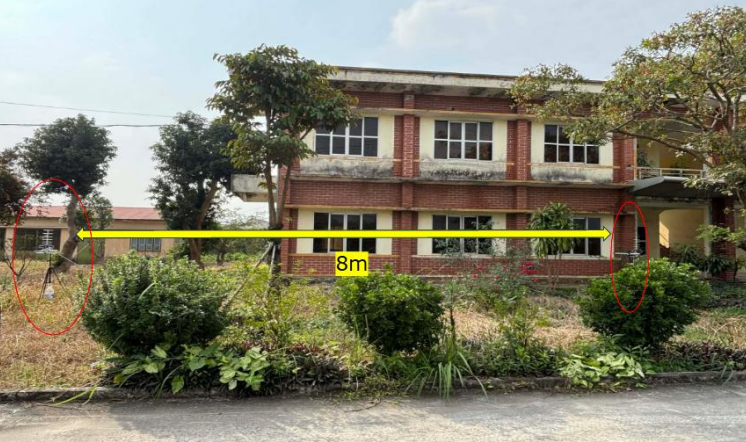
\includegraphics[width=\linewidth]{figs/photo_xuan_mai_field.png}\\
\small Two-element field deployment (Dec.\ 2025).
\end{columns}
\end{frame}

\begin{frame}{Problem Statement}
\begin{itemize}
  \item An ambiguous field result can come from \emph{several} causes at once:
  bad receivers, cable loss, RFI, weak geometry, or a genuinely weak signal.
  \item Without a reference model, these causes cannot be separated \emph{after the fact}.
\end{itemize}
\begin{alertblock}{Research Question}
How can a physically grounded, end-to-end simulation be built to evaluate the
feasibility, signal chain, and array-geometry choices of a low-cost UHF solar
radio interferometer \textbf{before} hardware deployment?
\end{alertblock}
\end{frame}

\begin{frame}{Objectives}
\begin{enumerate}
  \item \textbf{Antenna modelling:} 4NEC2 Method-of-Moments model of the Yagi-Uda
  element; cross-check against direct measurement.
  \item \textbf{End-to-end signal pipeline:} real flux $\to$ voltage $\to$
  visibility $\to$ dirty image, in Python.
  \item \textbf{General array geometry:} an ENU$\to$XYZ$\to uvw$ transform that
  works for \emph{any} 2-D layout, not just one fixed line.
  \item \textbf{Validation:} reproduce the classical analytic results (fringe
  period, $\jinc$-shaped visibility, dirty image) against a real transit.
\end{enumerate}
\end{frame}

% ============================================================
\section{Theoretical Background}

\begin{frame}{Solar Radio Bursts: Types I--V}
\begin{columns}[c]
\column{.55\textwidth}
\begin{itemize}
  \item Superimposed on the quiet-Sun thermal background, transient bursts can
  raise the flux by \textbf{orders of magnitude}.
  \item \textbf{Type I}: long-lived, narrowband noise storms.
  \item \textbf{Type III}: fast-drifting, electron beams on open field lines
  --- dominant at decimetre wavelengths.
  \item \textbf{Type II}: slowly drifting, traces coronal shock fronts (CMEs).
  \item \textbf{Type IV}: broadband continuum following flares.
\end{itemize}
\column{.45\textwidth}
\centering
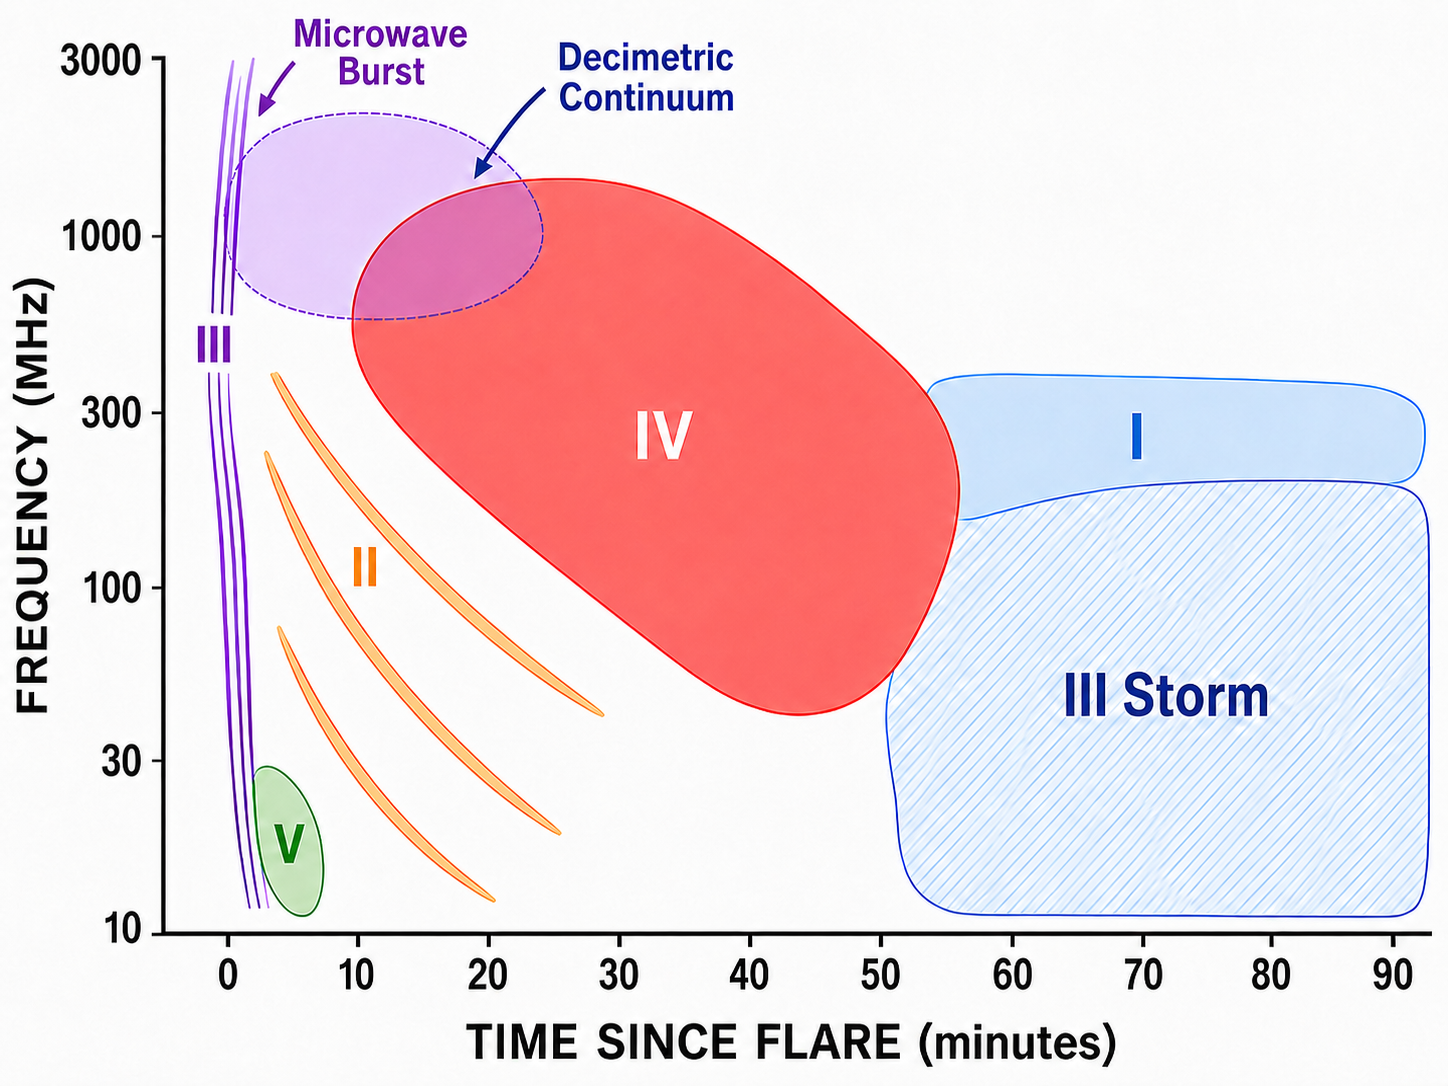
\includegraphics[width=\linewidth]{figs/fig_solar_dynamic_spectrum.png}
\end{columns}
\vspace{4pt}
\small Adapted from McLean \& Labrum and Dulk~\cite{dulk1985}.
\end{frame}

\begin{frame}{From Flux to Voltage}
\textbf{Friis reception relation:}
\[
P_{\rm sig} = \tfrac{1}{2} A_e\, S_\nu\, \Delta\nu, \qquad A_e = \frac{\lambda^2 G}{4\pi}
\]
\begin{itemize}
  \item $S_\nu$: incident flux density (solar flux units, sfu)~\cite{friis1946}
  \item $A_e$: antenna effective aperture, from the simulated gain $G$
  \item Received power is converted to an equivalent voltage:
  $V_{\rm rms} = \sqrt{P_{\rm rx} R_{\rm load}}$
\end{itemize}
\end{frame}

\begin{frame}{Receiver Noise \& the Radiometer Equation}
\textbf{Johnson-Nyquist thermal noise:}
\[
P_n = k_B\, T_{\rm sys}\, \Delta\nu
\]
\begin{itemize}
  \item Every receiver adds unavoidable thermal noise~\cite{nyquist1928}, set
  by the system temperature $T_{\rm sys}$.
  \item Averaging $N_s$ samples improves SNR by $\sqrt{N_s}$ (radiometer equation) ---
  the basis for detecting a weak solar signal in noise.
\end{itemize}
\end{frame}

\begin{frame}{Correlator, Visibility, and van Cittert--Zernike}
\begin{columns}[c]
\column{.42\textwidth}
\begin{itemize}
  \small
  \item A single antenna measures only power. Two antennas' voltages are
  cross-correlated into a complex \textbf{visibility}:
  $V_{ij} = \langle v_i\, v_j^{*}\rangle$
  \item The correlated signal traces \textbf{interference fringes} on the
  sky: their orientation and spacing are set purely by the baseline
  geometry and length ($\lambda/B$ rad).
  \item The van Cittert--Zernike theorem relates this fringe pattern
  $V(u,v)$ to the sky brightness $I(l,m)$ via a Fourier transform~\cite{tms2017}.
\end{itemize}
\column{.55\textwidth}
\centering
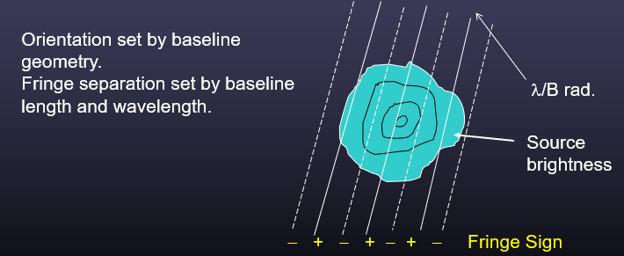
\includegraphics[width=\linewidth]{figs/fig_fringe_pattern.png}
\end{columns}
\end{frame}

\begin{frame}{Aperture Synthesis Imaging}
\begin{itemize}
  \item $(u,v,w)$: baseline expressed in wavelengths --- the spatial-frequency
  coordinate sampled by the array as the Earth rotates.
  \item Inverting the sampled visibilities by a Fourier transform gives the
  \textbf{dirty image}:
  \[
    I^{D} = I^{\rm sky} \ast B^{D}
  \]
  where $B^D$ is the synthesised beam (point-spread function, PSF).
  \item More/better-distributed baselines $\Rightarrow$ narrower PSF, better resolution.
\end{itemize}
\end{frame}

% ============================================================
\section{Antenna Design}

\begin{frame}{Yagi-Uda Antenna: 4NEC2 Model}
\begin{columns}[c]
\column{.48\textwidth}
\centering
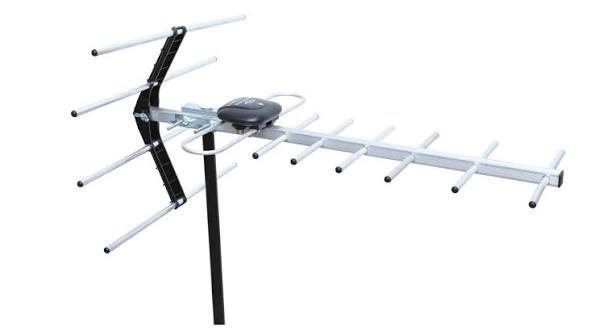
\includegraphics[width=\linewidth]{figs/photo_hkd_antenna.jpg}\\
\small Physical HKD~G11KD-T2 element.
\column{.48\textwidth}
\centering
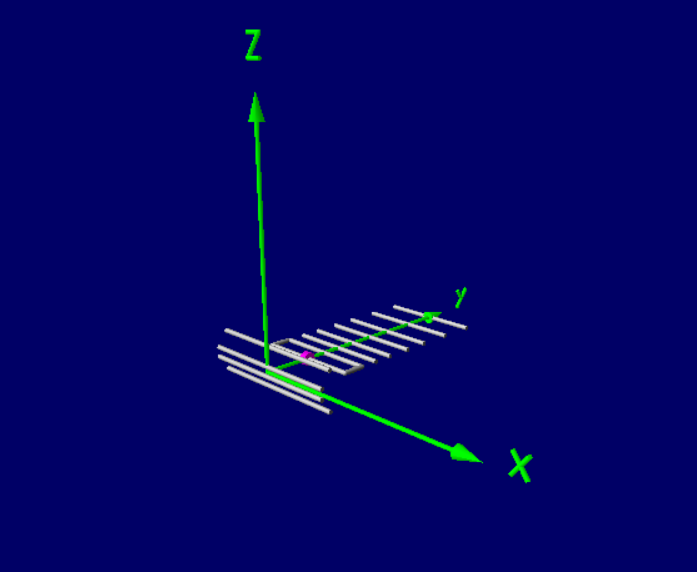
\includegraphics[width=\linewidth]{figs/fig_4nec2_wiremodel.png}\\
\small Method-of-Moments wire model (4NEC2)~\cite{nec2}.
\end{columns}
\vspace{6pt}
\begin{itemize}
  \item Commercial folded-dipole Yagi-Uda, six directors, U-frame reflector.
  \item Modelled wire-by-wire in 4NEC2 to extract impedance, gain, and pattern.
\end{itemize}
\end{frame}

\begin{frame}{Simulated Single-Element Performance}
\begin{columns}[c]
\column{.5\textwidth}
\begin{table}
\footnotesize
\begin{tabular}{lc}
\toprule
\textbf{Quantity} & \textbf{Value} \\
\midrule
Input impedance & $108.4 - j22.0\;\Omega$ \\
Forward gain & 9.48 dBi \\
Half-power beamwidth & $\approx 52^\circ$ \\
SWR (at 75~$\Omega$) & 1.55 \\
\bottomrule
\end{tabular}
\end{table}
\begin{itemize}
  \item Real part close to 75~$\Omega$ coax $\Rightarrow$ good match without a
  balun network.
\end{itemize}
\column{.5\textwidth}
\centering
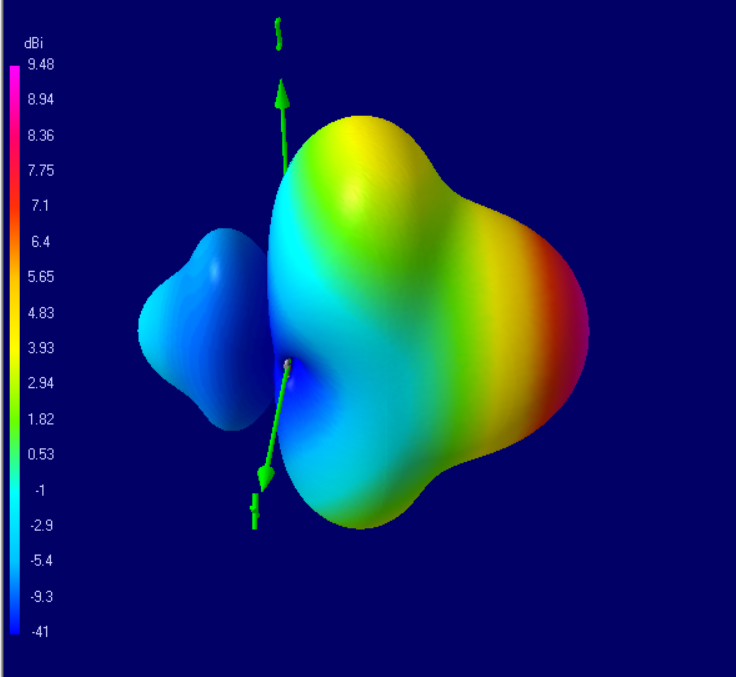
\includegraphics[width=\linewidth]{figs/fig_3d_radiation_pattern.png}\\
\small 3-D directivity pattern at 610~MHz.
\end{columns}
\end{frame}

\begin{frame}{Hardware Validation: NanoVNA vs.\ Simulation}
\begin{columns}[c]
\column{.5\textwidth}
\centering
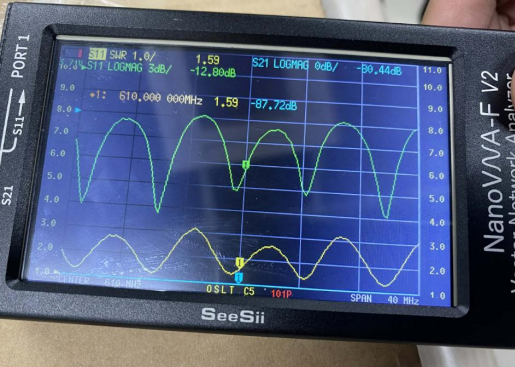
\includegraphics[width=\linewidth]{figs/photo_nanovna_setup.png}\\
\small NanoVNA measurement at the antenna feed point.
\column{.5\textwidth}
\begin{table}
\footnotesize
\centering
\begin{tabular}{lcc}
\toprule
\textbf{Method} & \textbf{SWR} & \makecell{\textbf{Return}\\\textbf{loss}} \\
\midrule
NanoVNA & 1.59 & $\approx-12.8$~dB \\
4NEC2   & 1.55 & $\approx-13.3$~dB \\
\bottomrule
\end{tabular}
\end{table}
\begin{itemize}
  \item Independent finite-element solution agrees within the same narrow range.
  \item Simulated pattern is trustworthy enough to drive the imaging pipeline.
\end{itemize}
\end{columns}
\end{frame}

\begin{frame}{Mutual Coupling Study}
\centering
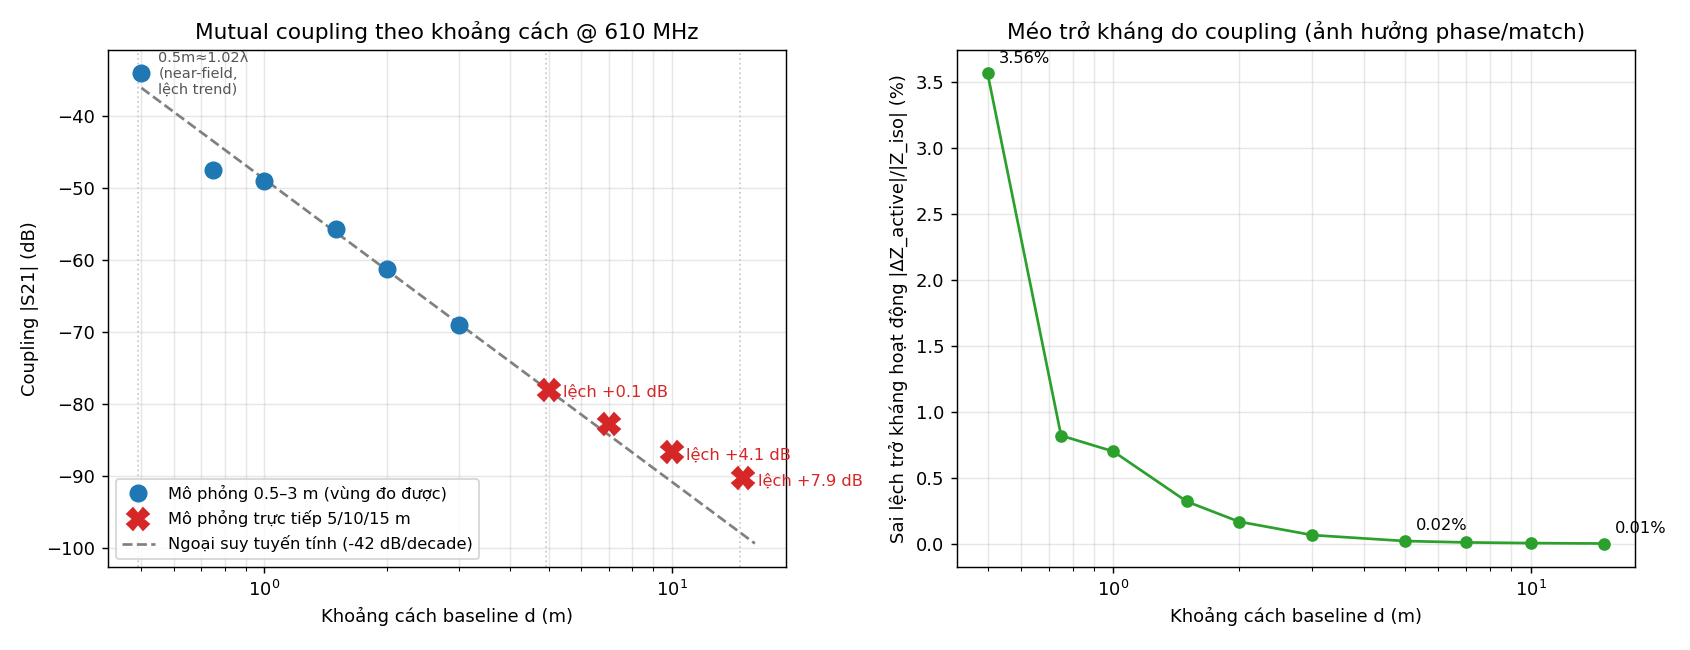
\includegraphics[width=0.95\linewidth]{figs/fig_coupling_curve.png}
\begin{itemize}
  \item Coupling falls from $-34$~dB at 0.5~m to below $-78$~dB by 5~m, and
  below $-87$~dB by 10~m.
  \item[$\Rightarrow$] Antennas behave as \textbf{independent sensors} at the
  operating baselines used in this thesis (8~m and above).
\end{itemize}
\end{frame}

% ============================================================
\section{Simulation Pipeline}

\begin{frame}{Pipeline Overview: Engine A --- Voltage Synthesis}
\centering
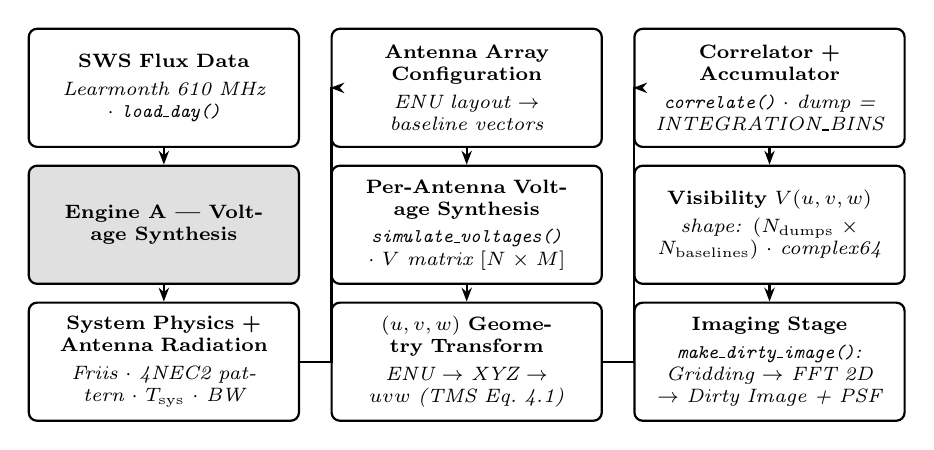
\begin{tikzpicture}[
  proc/.style={rectangle, rounded corners=3pt, draw=black, thick, fill=white,
               text width=3.15cm, align=center, inner sep=4pt, minimum height=1.5cm,
               font=\scriptsize},
  hdr/.style={proc, fill=black!12, font=\scriptsize\bfseries},
  arr/.style={-{Stealth[length=5pt]}, thick}
]
% Column 1
\node[proc] (data) {\textbf{SWS Flux Data}\\[2pt]{\itshape Learmonth 610~MHz $\cdot$ \texttt{load\_day()}}};
\node[hdr, below=6pt of data] (hdrA) {Engine A --- Voltage Synthesis};
\node[proc, below=6pt of hdrA] (phys) {\textbf{System Physics + Antenna Radiation}\\[2pt]{\itshape Friis $\cdot$ 4NEC2 pattern $\cdot$ $T_{\mathrm{sys}}$ $\cdot$ BW}};

% Column 2
\node[proc, right=11pt of data] (arrcfg) {\textbf{Antenna Array Configuration}\\[2pt]{\itshape ENU layout $\to$ baseline vectors}};
\node[proc, below=6pt of arrcfg] (volt) {\textbf{Per-Antenna Voltage Synthesis}\\[2pt]{\itshape \texttt{simulate\_voltages()} $\cdot$ $V$ matrix $[N\times M]$}};
\node[proc, below=6pt of volt] (geom) {\textbf{$(u,v,w)$ Geometry Transform}\\[2pt]{\itshape ENU $\to$ XYZ $\to$ $uvw$ (TMS Eq.~4.1)}};

% Column 3
\node[proc, right=11pt of arrcfg] (corr) {\textbf{Correlator + Accumulator}\\[2pt]{\itshape \texttt{correlate()} $\cdot$ dump = INTEGRATION\_BINS}};
\node[proc, below=6pt of corr] (vis) {\textbf{Visibility $V(u,v,w)$}\\[2pt]{\itshape shape: $(N_{\rm dumps}\times N_{\rm baselines})$ $\cdot$ complex64}};
\node[proc, below=6pt of vis] (img) {\textbf{Imaging Stage}\\[2pt]{\itshape \texttt{make\_dirty\_image()}: Gridding $\to$ FFT~2D $\to$ Dirty Image + PSF}};

% Vertical flow within each column
\draw[arr] (data) -- (hdrA);
\draw[arr] (hdrA) -- (phys);
\draw[arr] (arrcfg) -- (volt);
\draw[arr] (volt) -- (geom);
\draw[arr] (corr) -- (vis);
\draw[arr] (vis) -- (img);

% Column-to-column wrap connectors
\draw[arr] (phys.east) -- ++(0.4,0) |- (arrcfg.west);
\draw[arr] (geom.east) -- ++(0.4,0) |- (corr.west);
\end{tikzpicture}

\vspace{4pt}
\footnotesize Full per-antenna signal chain, realistic SNR --- used for physical validation.
\end{frame}

\begin{frame}{Pipeline Overview: Engine B --- Analytic Cross-Check}
\begin{columns}[c]
\column{.42\textwidth}
\centering
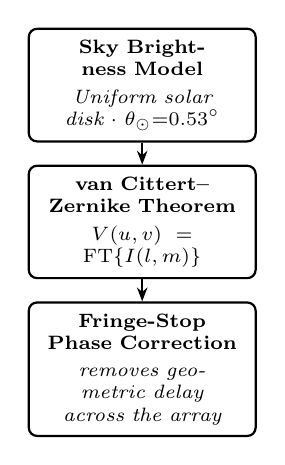
\begin{tikzpicture}[
  proc/.style={rectangle, rounded corners=3pt, draw=black, thick, fill=white,
               text width=2.6cm, align=center, inner sep=4pt, minimum height=1.3cm,
               font=\scriptsize},
  arr/.style={-{Stealth[length=5pt]}, thick}
]
\node[proc] (sky) {\textbf{Sky Brightness Model}\\[2pt]{\itshape Uniform solar disk $\cdot$ $\theta_\odot{=}0.53^\circ$}};
\node[proc, below=8pt of sky] (vcz) {\textbf{van Cittert--Zernike Theorem}\\[2pt]{\itshape $V(u,v) = \mathrm{FT}\{I(l,m)\}$}};
\node[proc, below=8pt of vcz] (fs) {\textbf{Fringe-Stop Phase Correction}\\[2pt]{\itshape removes geometric delay across the array}};
\draw[arr] (sky) -- (vcz);
\draw[arr] (vcz) -- (fs);
\end{tikzpicture}
\column{.54\textwidth}
\centering
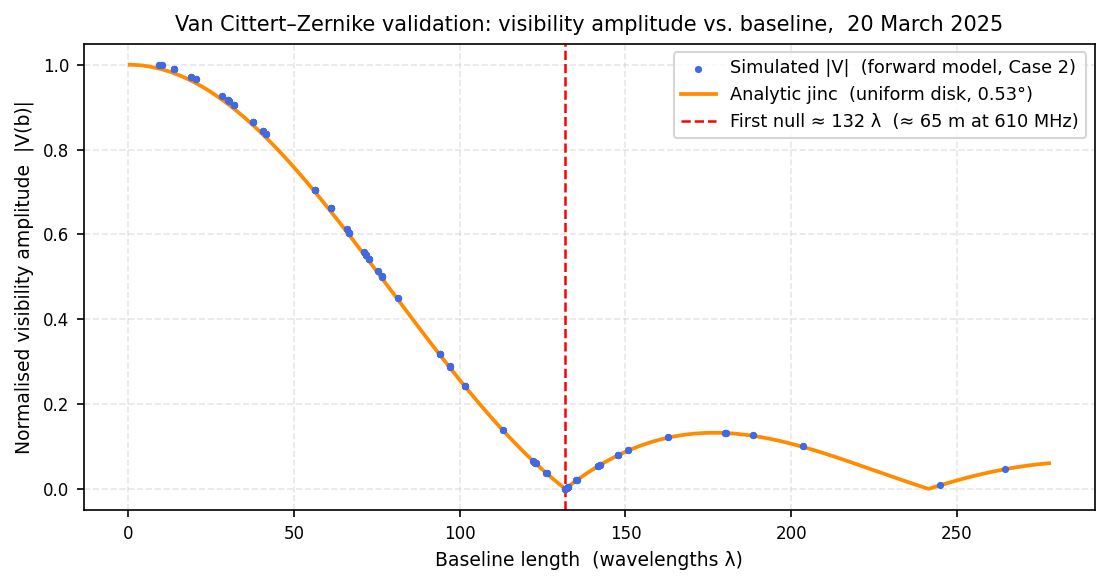
\includegraphics[width=\linewidth]{figs/fig_visibility_jinc.png}
\end{columns}
\vspace{4pt}
\begin{itemize}
  \footnotesize
  \item Fast, closed-form analytic model --- \emph{not} a full per-antenna signal chain.
  \item Used solely to cross-check Engine A's output against the theoretical
  jinc-shaped visibility curve.
\end{itemize}
\end{frame}

\begin{frame}{Input Data: Learmonth 610~MHz Flux Record}
\centering
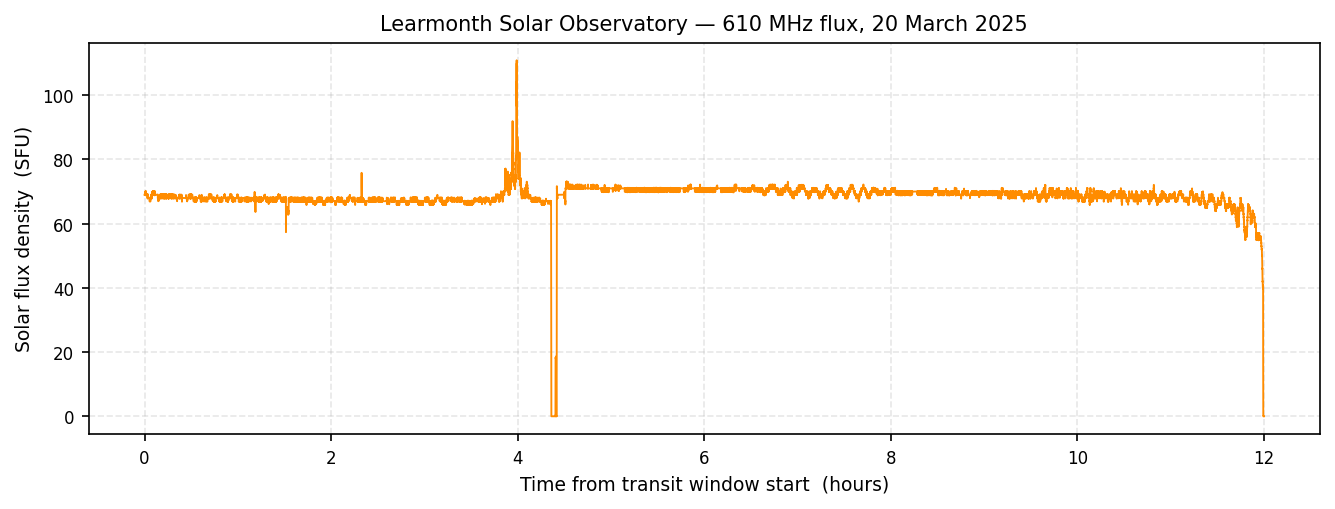
\includegraphics[width=0.92\linewidth]{figs/fig_sws_flux_day.png}

\vspace{4pt}
\begin{itemize}
  \small
  \item Real, archived daily flux from the SWS Learmonth Observatory,
  Australia~\cite{sws}.
  \item Used as an \emph{external}, already-calibrated flux input --- the
  simulation does not reproduce Learmonth's internal receiver.
  \item Transit date used throughout: 20 March 2025 (spring equinox, $\delta=0^\circ$).
\end{itemize}
\end{frame}

\begin{frame}{Voltage Synthesis \& Noise Injection}
\centering
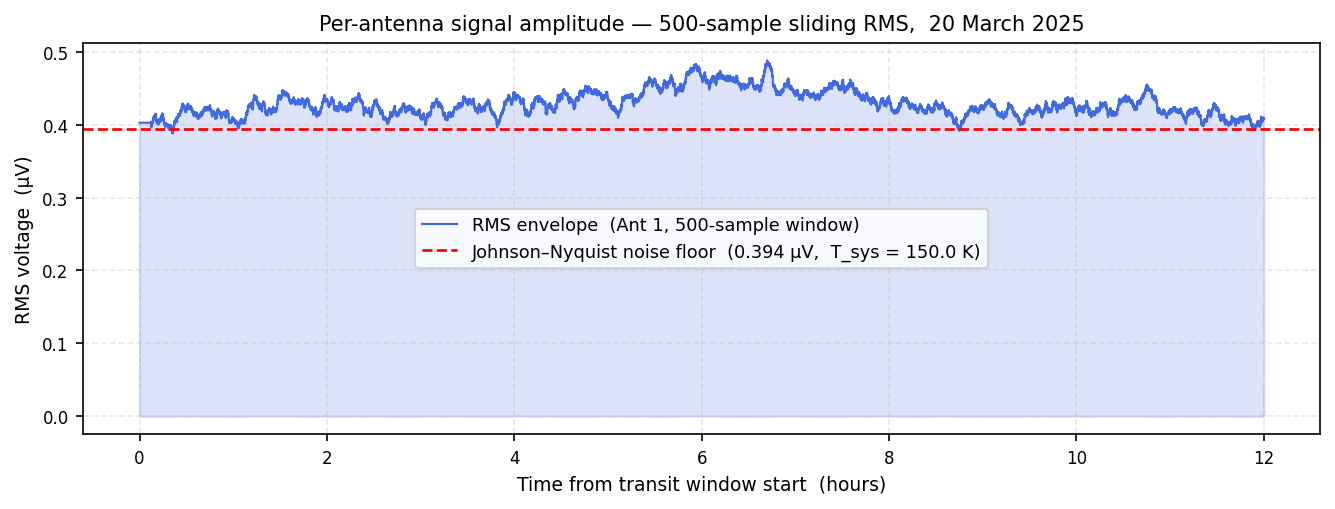
\includegraphics[width=0.88\linewidth]{figs/fig_voltage_env.png}
\begin{itemize}
  \item Flux $\to$ Friis power $\to$ equivalent voltage, with additive
  Johnson-Nyquist noise and the 4NEC2 primary beam applied along the solar track.
  \item Per-antenna complex baseband voltage, ready for correlation.
\end{itemize}
\end{frame}

\begin{frame}{Array Geometry: ENU $\to$ XYZ $\to uvw$}
\begin{columns}[c]
\column{.48\textwidth}
\centering
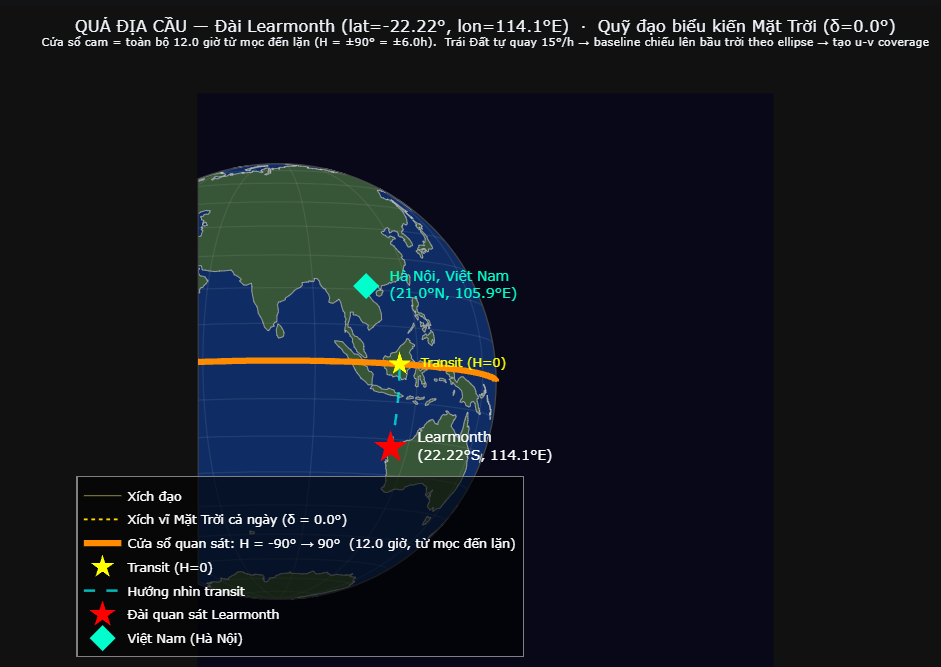
\includegraphics[width=\linewidth]{figs/fig_globe_track.png}\\
\small Apparent solar track over the 12-h transit.
\column{.48\textwidth}
\centering
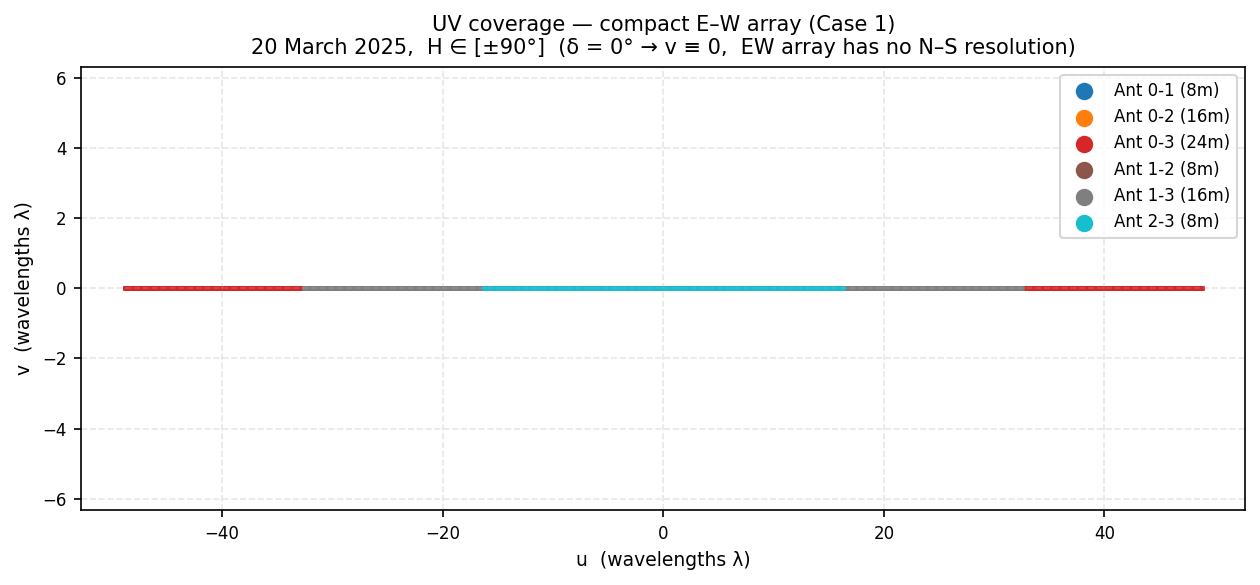
\includegraphics[width=\linewidth]{figs/fig_uv_coverage.png}\\
\small Resulting $uv$-coverage.
\end{columns}
\vspace{6pt}
\begin{itemize}
  \item One consistent geometry transform works for \emph{any} 2-D array layout ---
  key to comparing multiple configurations fairly.
\end{itemize}
\end{frame}

\begin{frame}{Correlator \& Visibility Formation}
\begin{itemize}
  \item Antenna voltage pairs are cross-correlated and time-averaged into
  visibilities every $\approx 43.2$~s (integration dump).
  \item \textbf{Validation:} visibility amplitude at transit peak must decay
  as $\jinc(u\,\theta_\odot)$ with baseline length.
\end{itemize}
\centering
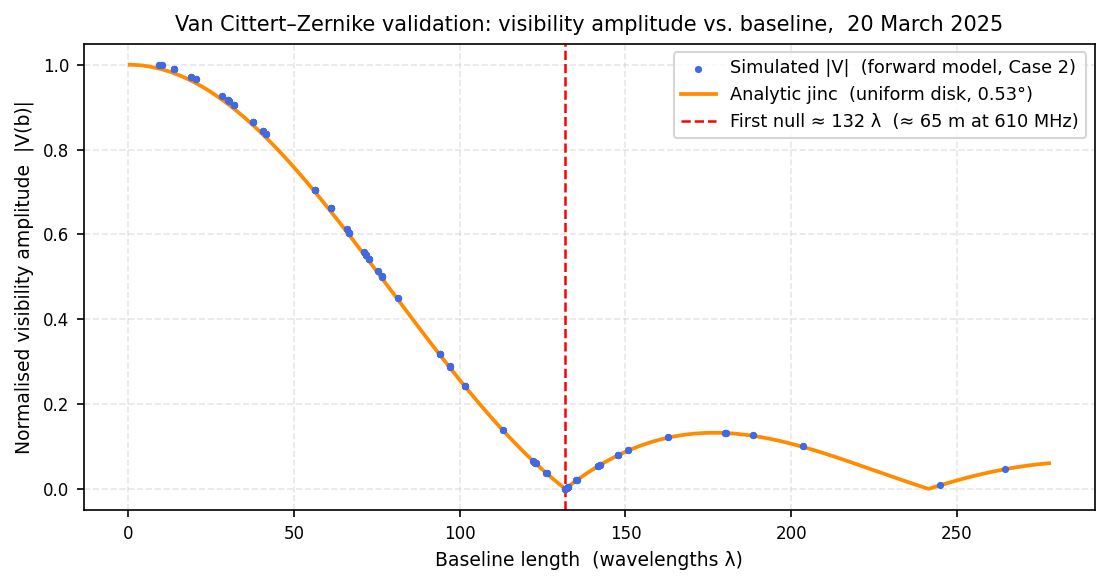
\includegraphics[width=0.88\linewidth]{figs/fig_visibility_jinc.png}
\end{frame}

\begin{frame}{Imaging: Dirty Image \& PSF Validation}
\centering
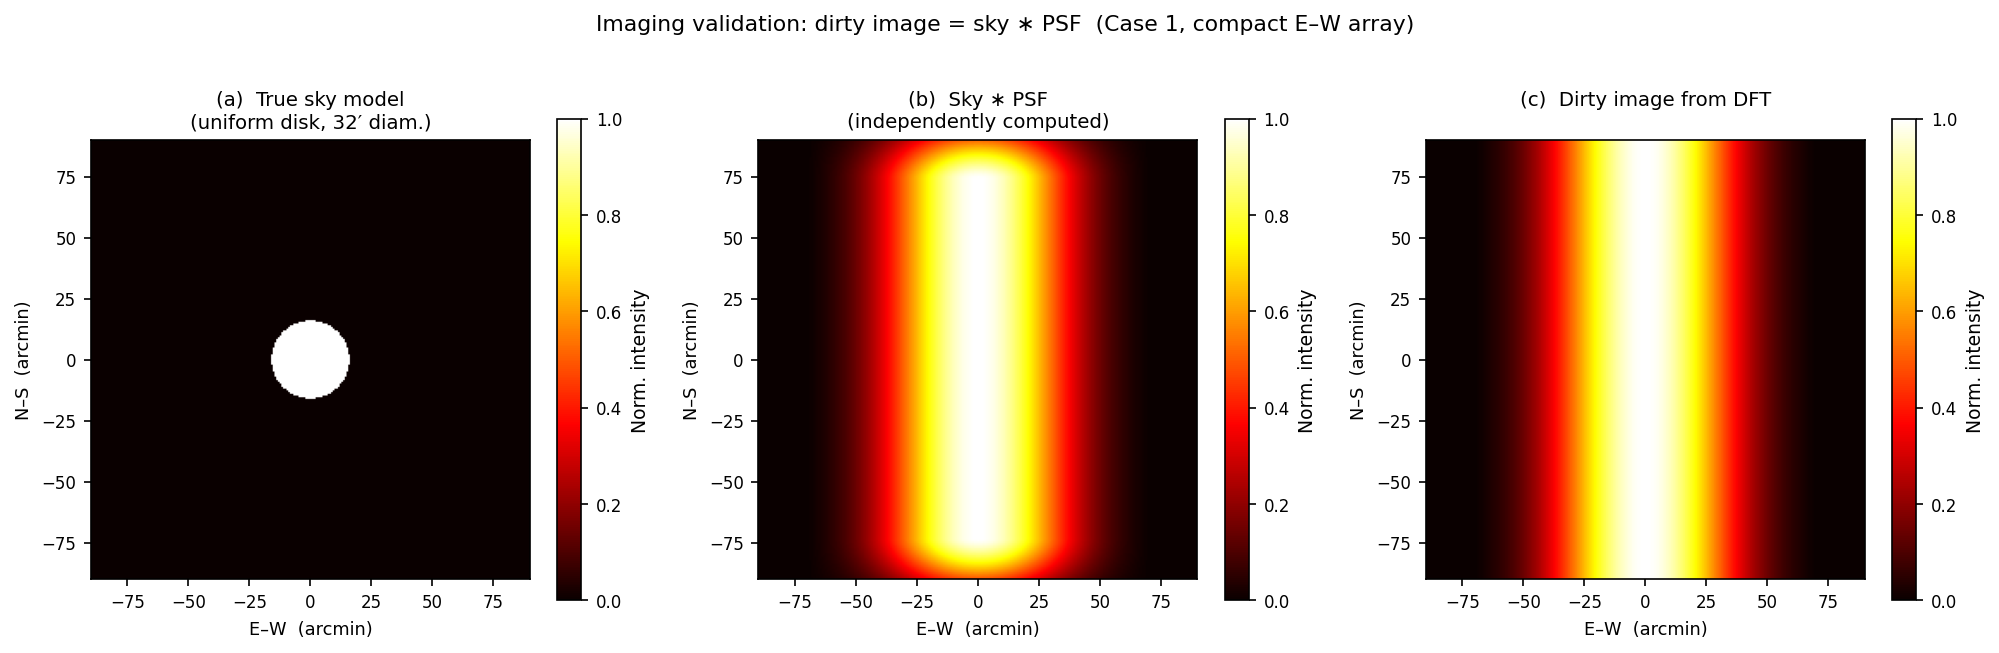
\includegraphics[width=0.98\linewidth]{figs/fig_sky_conv_psf.png}
\begin{itemize}
  \footnotesize
  \item The \textbf{dirty image} is \emph{not} the true sky: it is the true
  sky convolved with the array's \textbf{point-spread function (PSF)},
  $I^D = I^{\rm sky} \ast B^D$ --- panels (a)+(b).
  \item The PSF (``dirty beam'') is set purely by the $uv$-sampling
  pattern; its sidelobes are imaging artefacts from missing spatial
  frequencies, not real sky structure.
  \item Panel (c) is computed independently via gridding + FFT on the
  correlator output; agreement with (b) validates the imaging stage.
\end{itemize}
\end{frame}

% ============================================================
\section{Evaluation \& Results}

\begin{frame}{Evaluation Cases Overview}
\begin{table}
\footnotesize
\centering
\begin{tabular}{lll}
\toprule
\textbf{Case} & \textbf{Layout} & \textbf{Purpose} \\
\midrule
1    & Compact E-W, 4 ant.\ (24~m)     & Baseline detection, 1-D only \\
1.5  & Cross, 4 ant.\ (8~m unit)       & Recover 2-D resolution \\
1.75 & DLITE-inspired triangle+centre  & Non-redundant, minimal-antenna 2-D \\
2    & Extended graded cross (130~m)  & Resolve the solar disk \\
Sweep& 5 geometries                    & Systematic layout comparison \\
\bottomrule
\end{tabular}
\end{table}
\end{frame}

\begin{frame}{Case 1 \& 1.5: From One-Dimensional to Cross Baselines}
\begin{columns}[c]
\column{.4\textwidth}
\centering
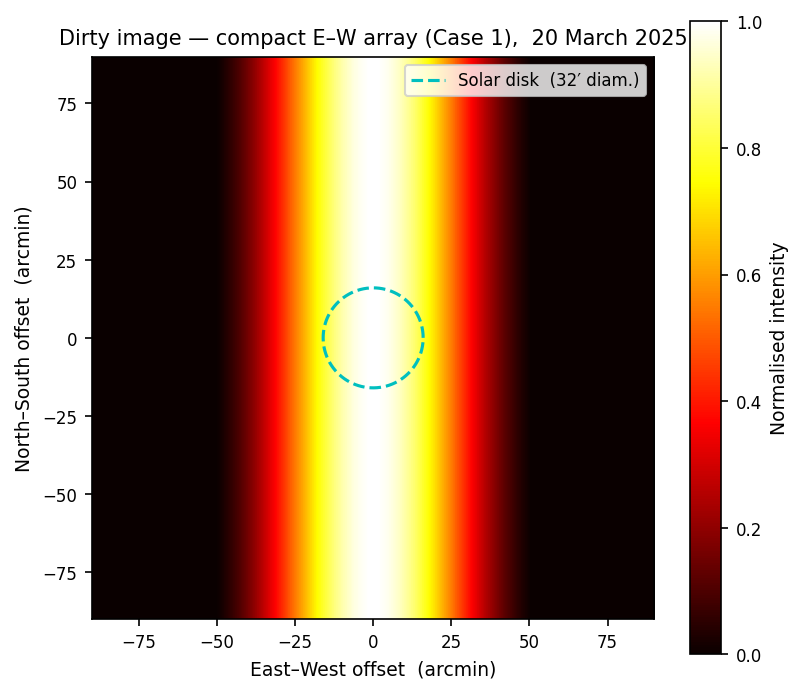
\includegraphics[width=\linewidth]{figs/fig_dirty_image.png}\\
\small Case~1: E-W-only, N-S smeared.
\column{.5\textwidth}
\centering
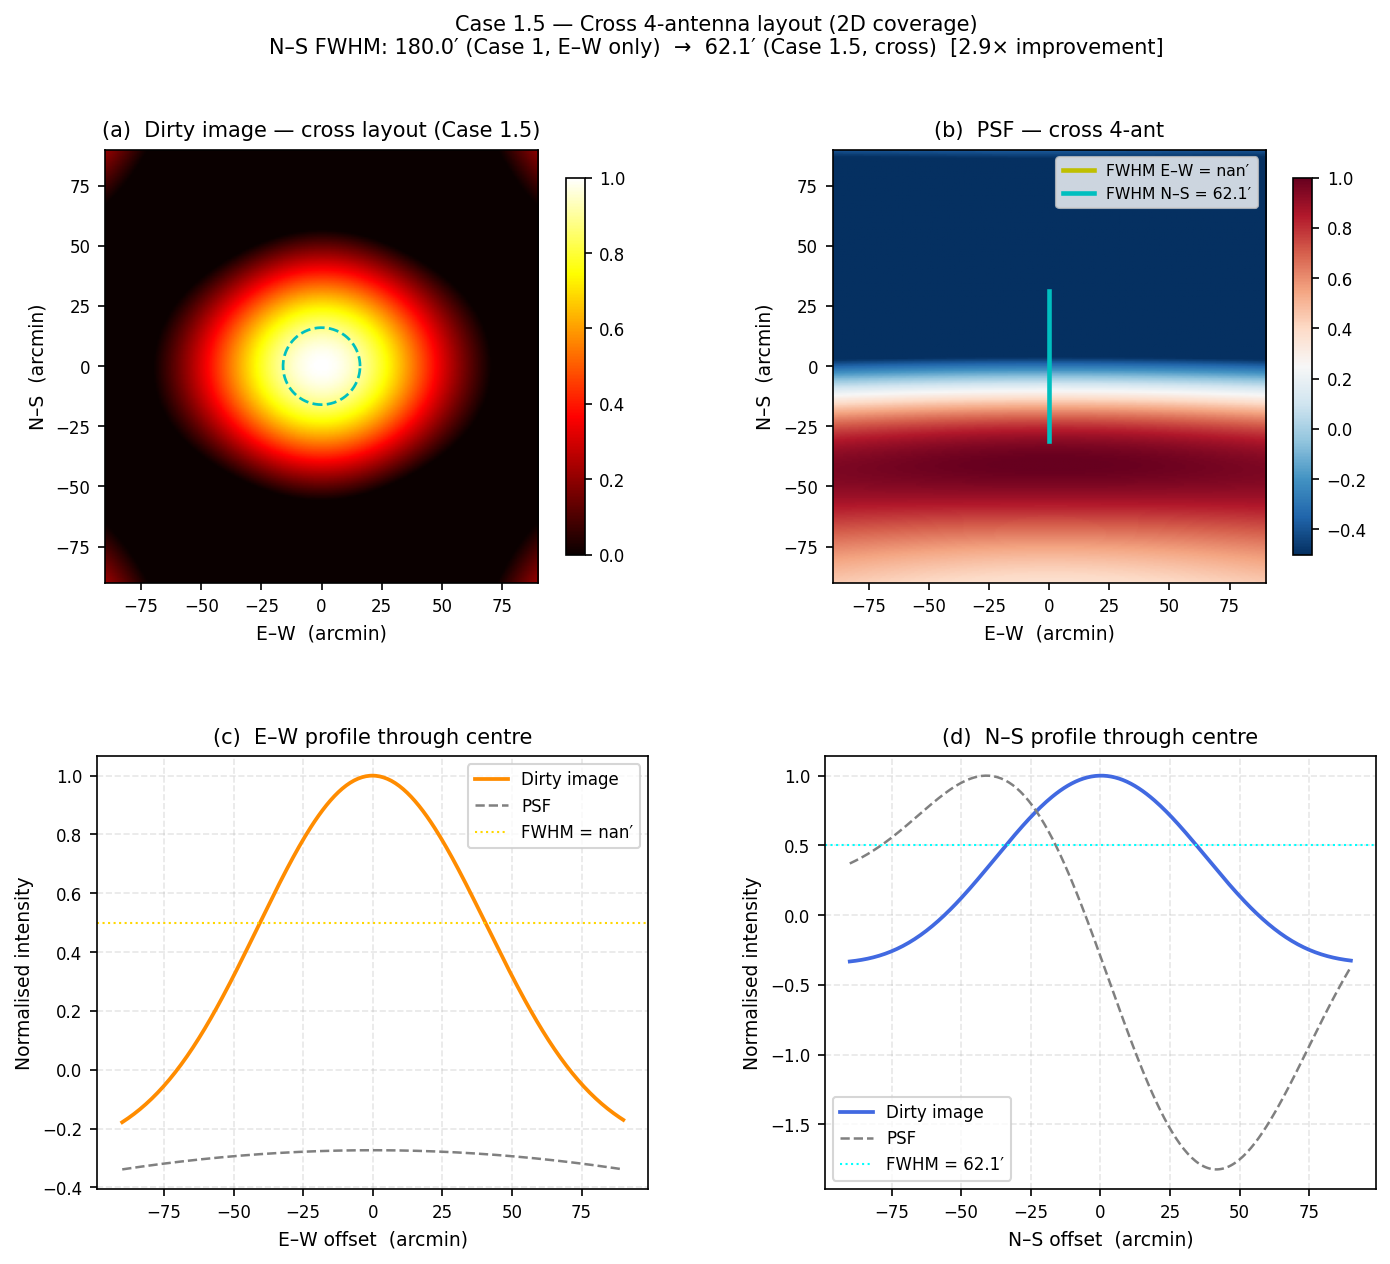
\includegraphics[width=\linewidth]{figs/fig_dirty_from_dft.png}\\
\small Case~1.5: cross layout.
\end{columns}
\vspace{-2pt}
\begin{table}
\footnotesize
\centering
\begin{tabular}{lccc}
\toprule
\textbf{Layout} & FWHM E-W & FWHM N-S & Ratio N-S/E-W \\
\midrule
Case 1 (E-W)   & $\sim 35'$ & $\gg 100'$ & $\gg 1$ \\
Case 1.5 (Cross) & $\sim 53'$ & $\sim 53'$ & $\approx 1$ \\
\bottomrule
\end{tabular}
\end{table}
\end{frame}

\begin{frame}{Case 1.75: DLITE-Inspired Minimum-Redundancy Layout}
\begin{columns}[c]
\column{.36\textwidth}
\centering
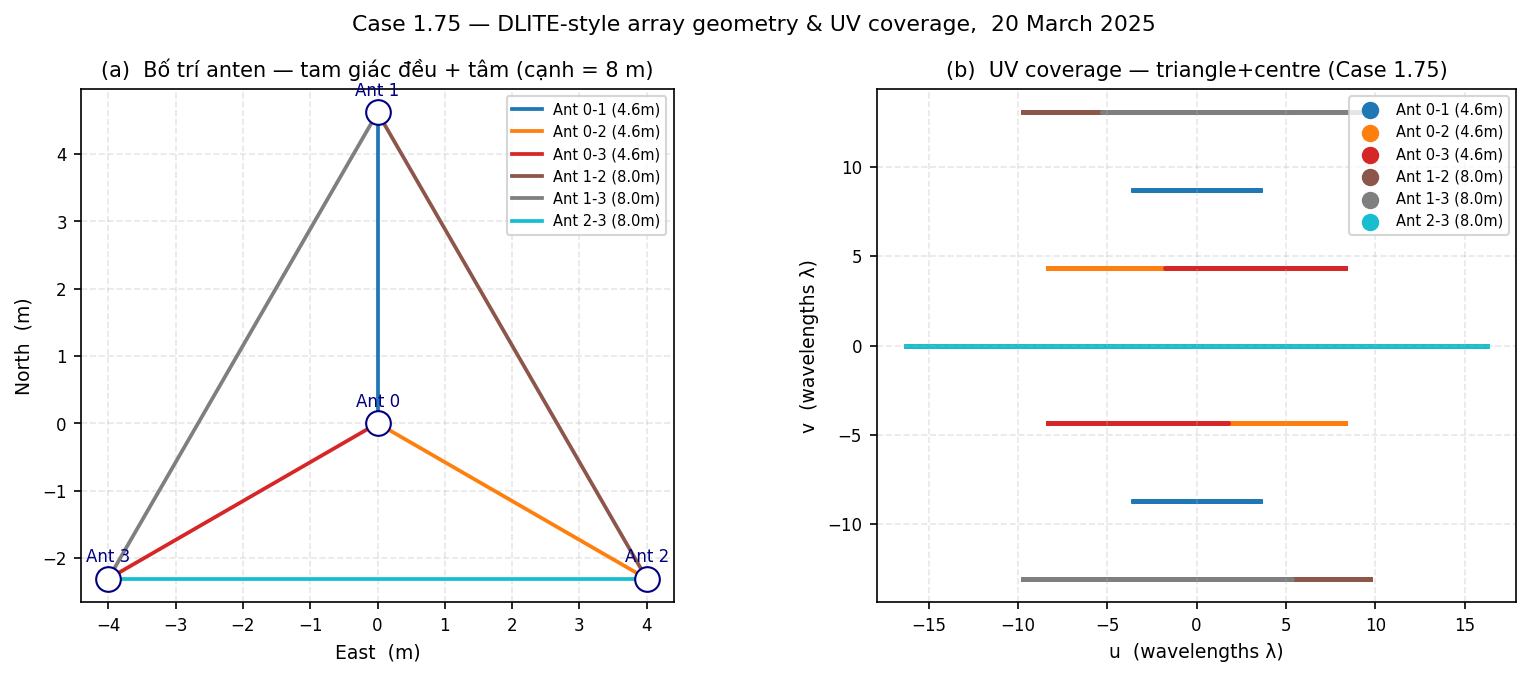
\includegraphics[width=\linewidth]{figs/fig_case175_geometry.png}
\column{.52\textwidth}
\centering
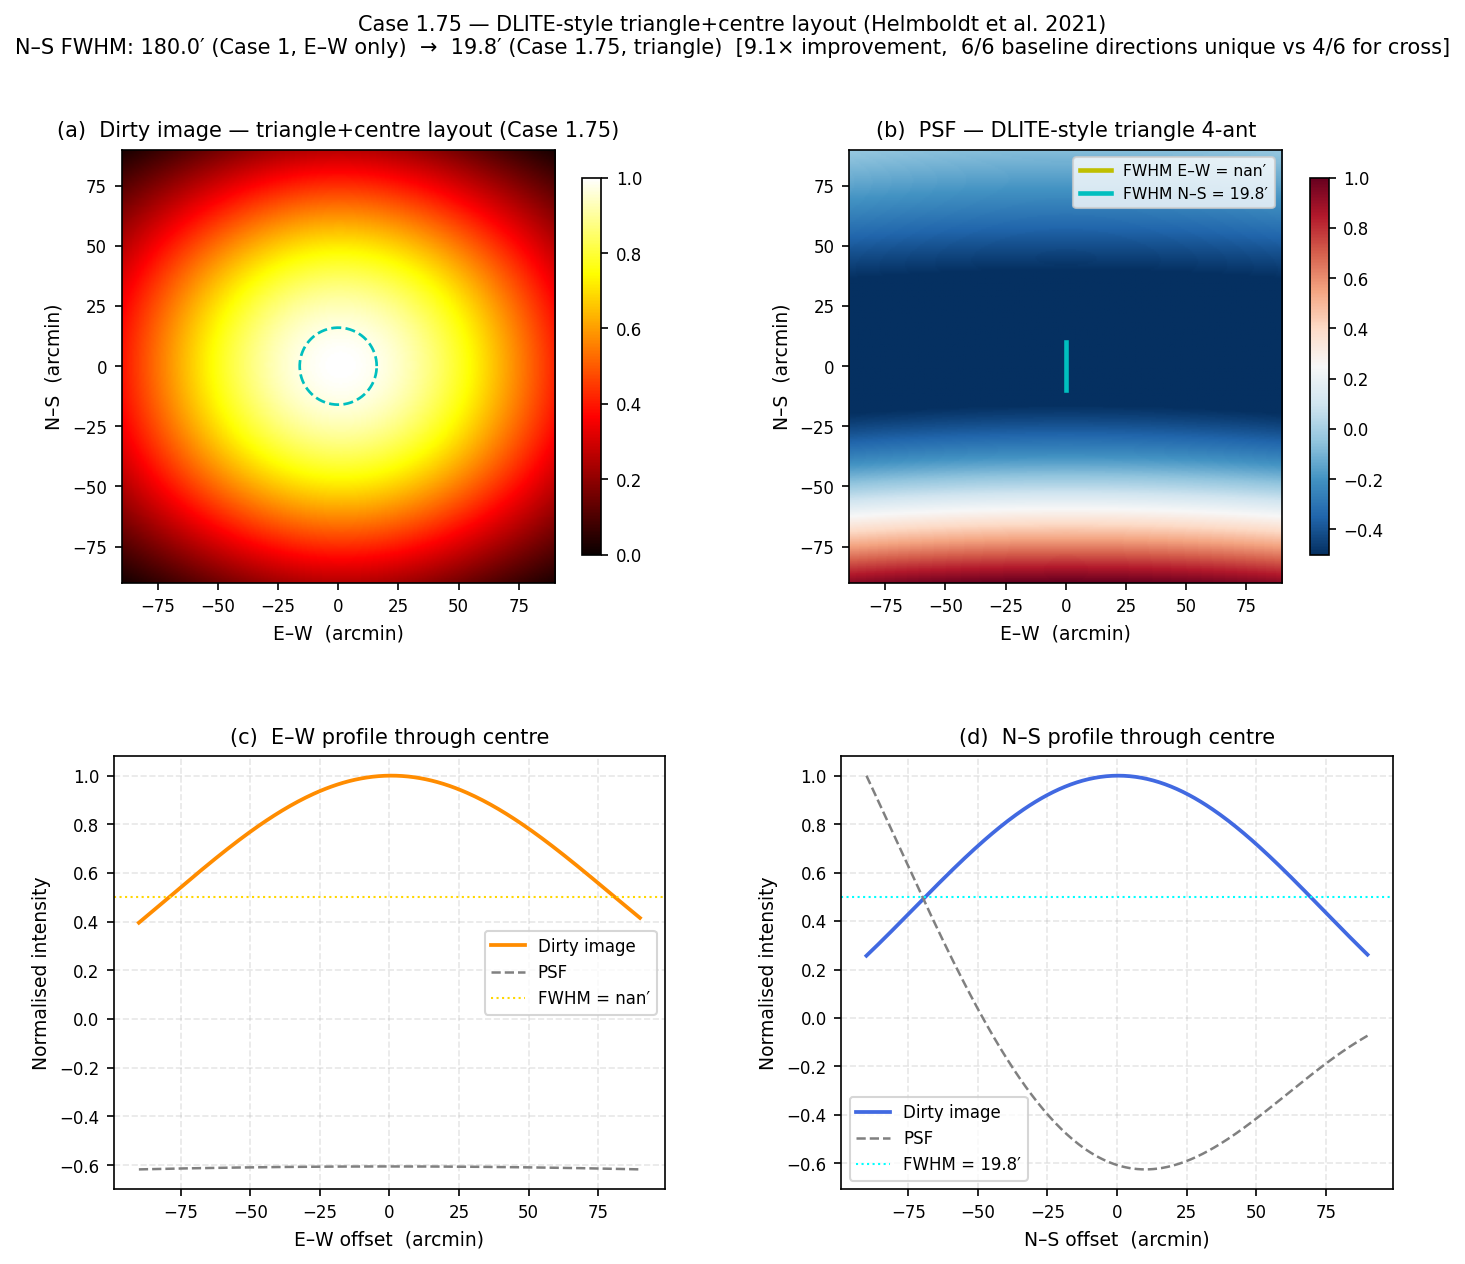
\includegraphics[width=\linewidth]{figs/fig_case175_eval.png}
\end{columns}
\vspace{2pt}
\footnotesize
\begin{itemize}
  \item Same four antennas, same 8~m spacing --- rearranged as a triangle plus
  a centre element, inspired by DLITE's minimum-redundancy
  philosophy~\cite{helmboldt2021dlite}.
  \item All six baselines point in \textbf{distinct} directions $\Rightarrow$
  North-South FWHM improves \textbf{9.1$\times$} versus Case~1.
  \item Not a full DLITE simulation: same topology, but at 610~MHz with an
  8~m scale, not DLITE's 30--40~MHz / hundreds-of-metres system.
\end{itemize}
\end{frame}

\begin{frame}{Case 2: Resolving the Solar Disk}
\centering
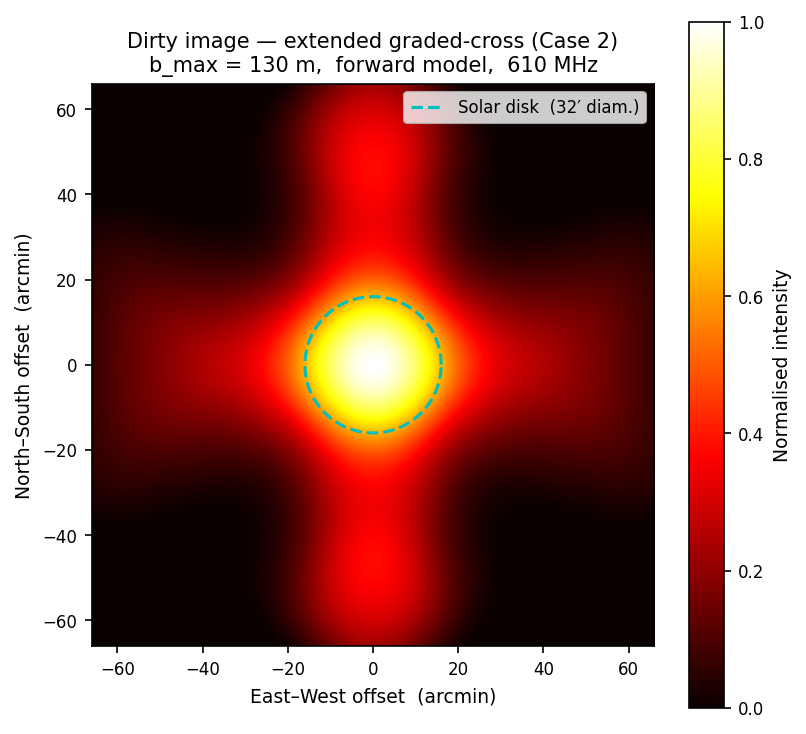
\includegraphics[width=0.5\linewidth]{figs/fig_case2_image.png}
\begin{itemize}
  \item Extended graded-cross array, baselines up to 130~m
  ($u_{\rm max}\approx 265\,\lambda$).
  \item E-W resolution $\approx 11'$ --- sufficient to begin resolving the
  $32'$ solar disk.
  \item Visibility amplitude drops below 50\% by $u\approx130\,\lambda$: the
  interferometric signature of a partially resolved source.
\end{itemize}
\end{frame}

\begin{frame}{Geometry Sweep: Five Array Layouts}
\centering
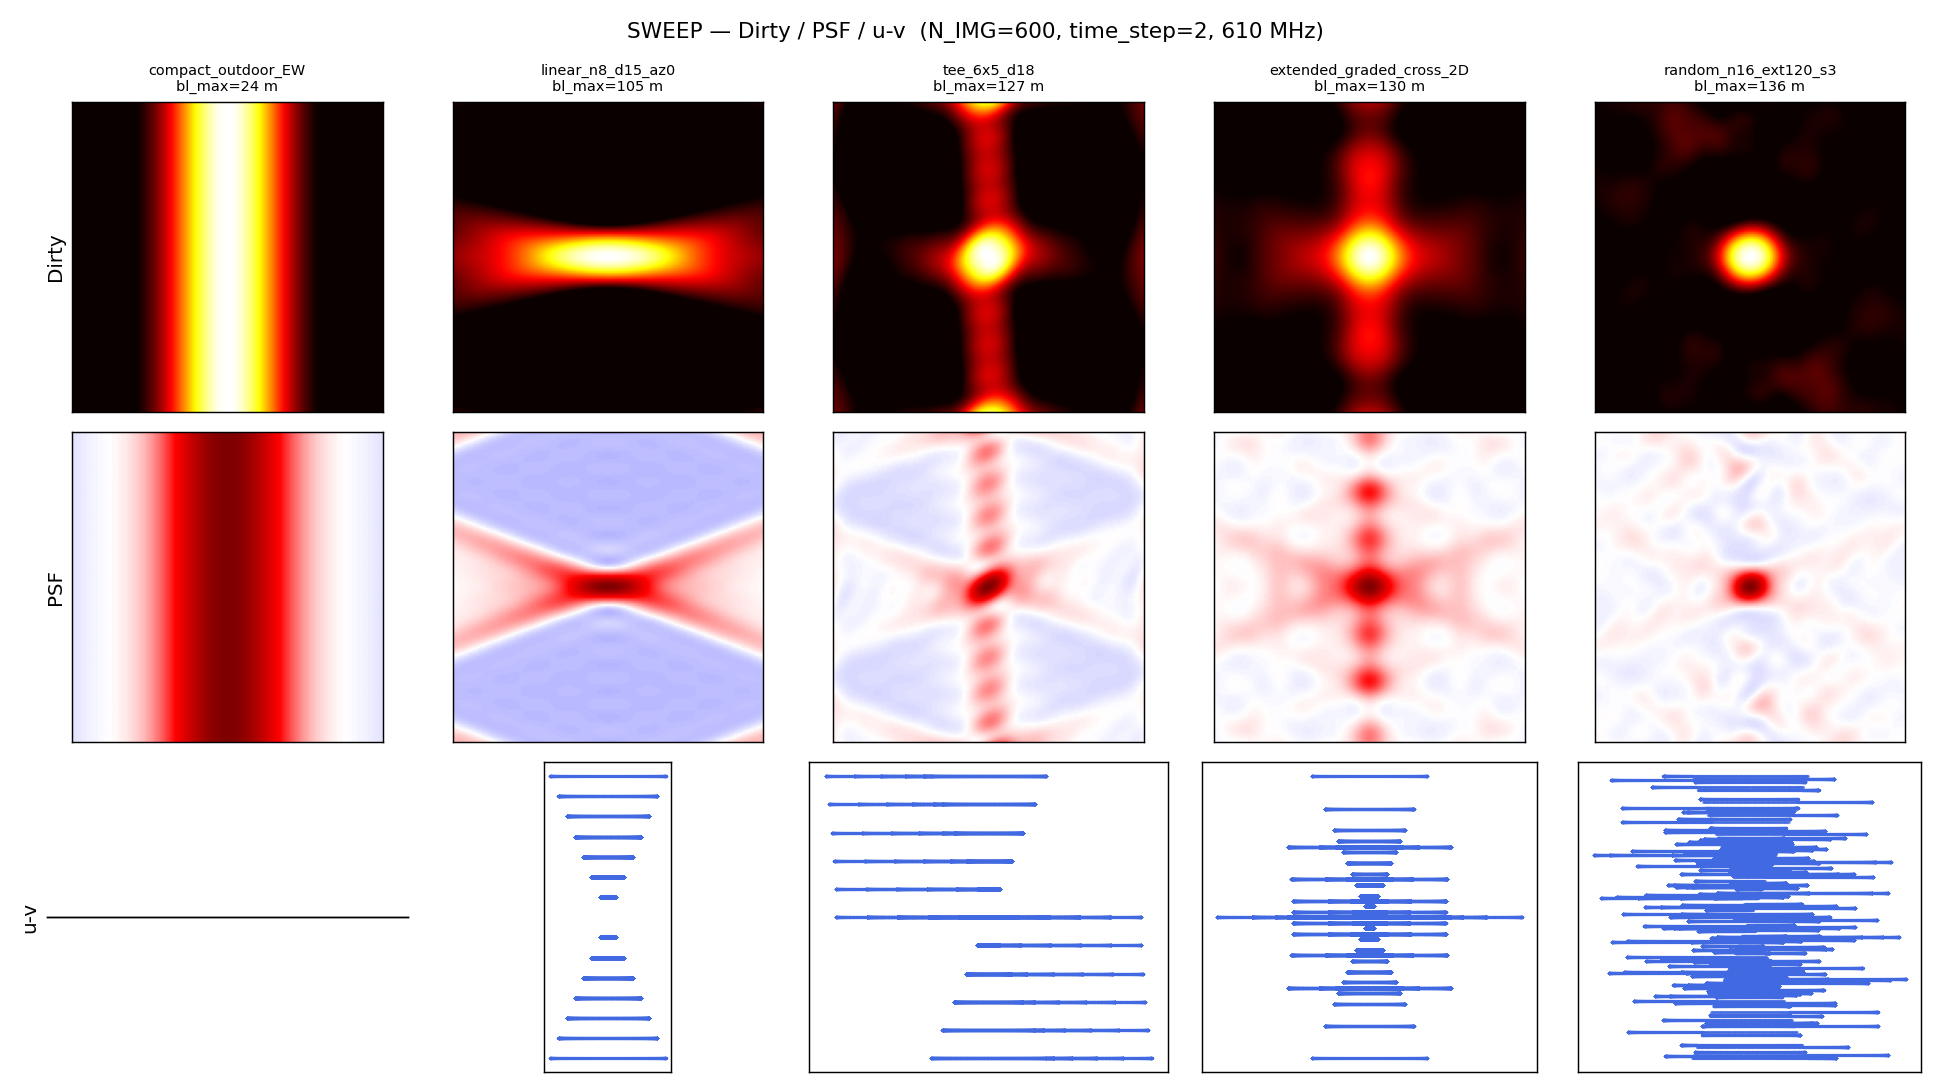
\includegraphics[width=\linewidth]{figs/fig_layout_sweep.png}
\small Compact E-W $\to$ N-S line $\to$ tee $\to$ extended cross $\to$ random 2-D:
longer, better-distributed baselines steadily improve resolution and sidelobe suppression.
\end{frame}

\begin{frame}{Sensitivity \& Burst Detectability}
\begin{itemize}
  \item Quiet-Sun signal alone reaches SNR $\approx 1{,}700$ per integration dump.
  \item Every burst category in the catalogue is detectable at extreme significance:
\end{itemize}
\begin{table}
\footnotesize
\centering
\begin{tabular}{lcc}
\toprule
\textbf{Event type} & \textbf{Flux (sfu)} & \textbf{SNR (1 dump)} \\
\midrule
Quiet Sun         & --              & $\approx 1{,}700$ \\
Type IV continuum & $\sim$200--1{,}000 & 3{,}400--17{,}200 \\
Type III (moderate) & $\sim$1{,}000 & $\sim$17{,}200 \\
Type II (shock)   & 500--5{,}000    & 8{,}600--86{,}000 \\
\bottomrule
\end{tabular}
\end{table}
\end{frame}

\begin{frame}{Hardware Comparison: Simulation vs.\ Measurement}
\begin{itemize}
  \item Simulated solar excess compared against the two-element analogue
  interferometer at Hoa Lac, Hanoi (20 March 2025, same transit date).
  \item A factor of \textbf{23.8$\times$} gap in SNR is found, attributed to
  the high effective system temperature of the consumer SDR receiver
  ($T_{\rm sys,eff}\approx 3{,}600$~K vs.\ the ideal $150$~K model).
\end{itemize}
\begin{alertblock}{Key finding}
The dominant gap between model and hardware is \textbf{system temperature},
not signal-chain modelling --- this directly guides hardware upgrade priorities.
\end{alertblock}
\end{frame}

\begin{frame}{Comparison with APSYNSIM}
\begin{itemize}
  \item APSYNSIM~\cite{apsynsim}: a widely used open-source aperture-synthesis
  teaching tool (Onsala Space Observatory).
  \item Uses synthetic sky models and a simplified Gaussian primary beam ---
  no real flux data, no real hardware pattern.
  \item[$\Rightarrow$] This work's pipeline adds real Learmonth flux, a
  measured 4NEC2 antenna pattern, and a real hardware comparison, at the cost
  of being tied to one physical scenario rather than a general teaching demo.
\end{itemize}
\end{frame}

\begin{frame}{Companion Tool: Browser-Based Interactive Simulator}
\centering
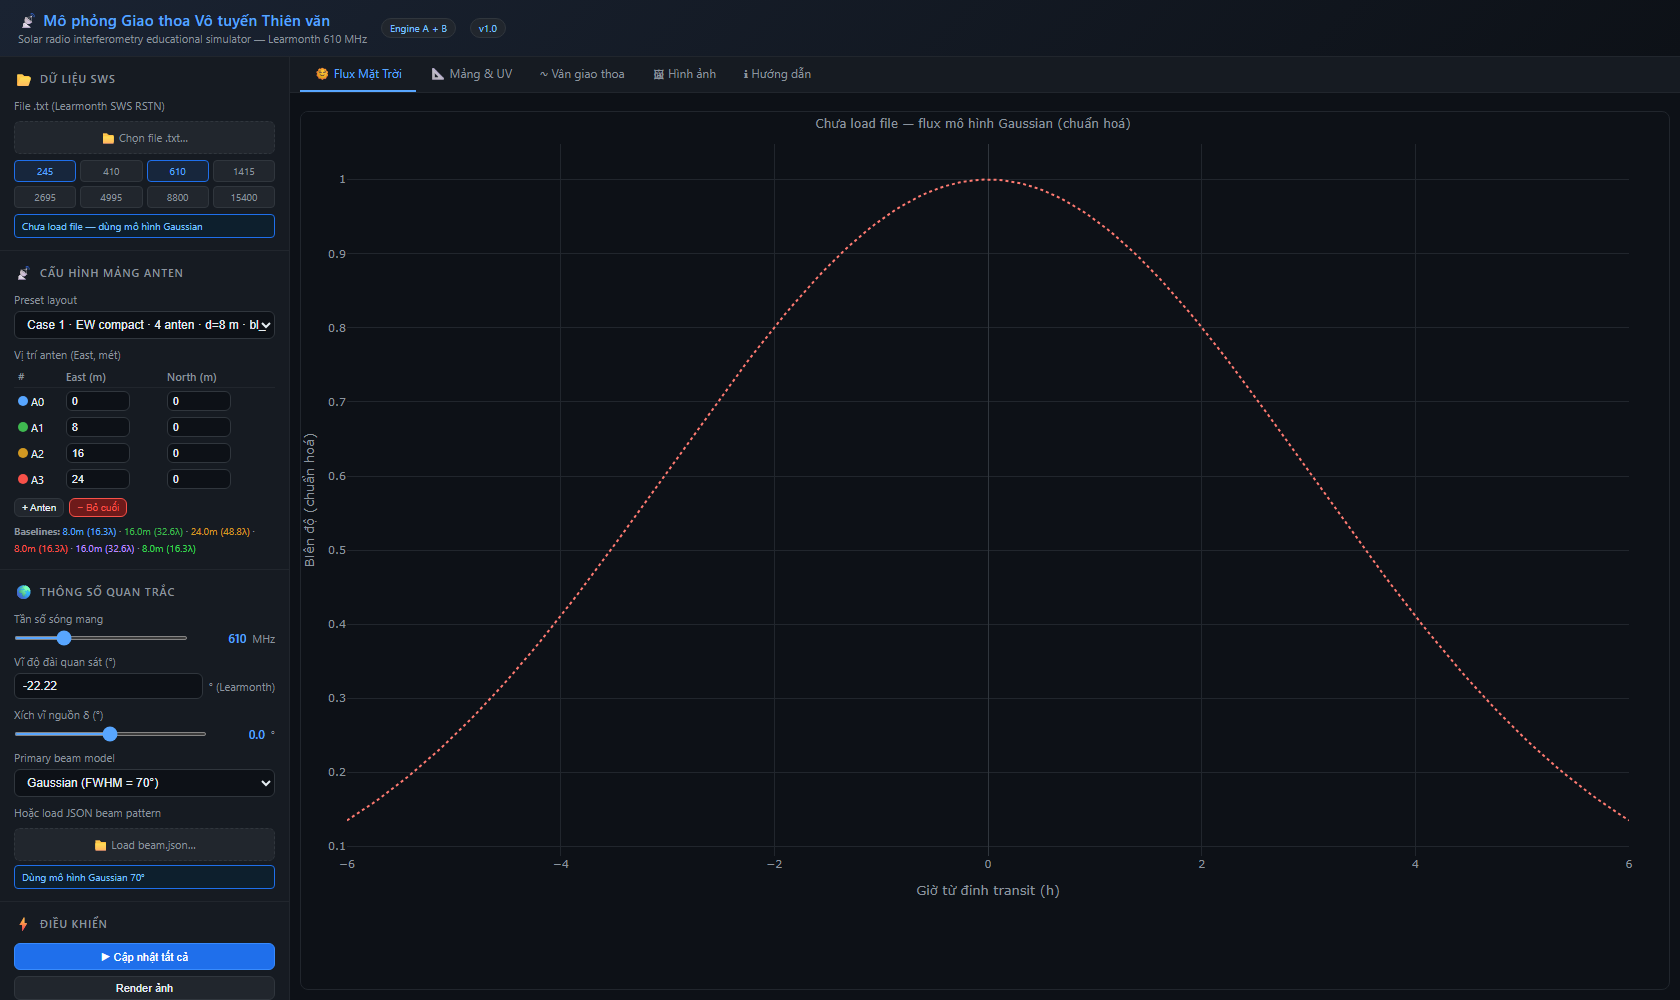
\includegraphics[width=0.68\linewidth]{figs/fig_html_tool_main.png}

\vspace{4pt}
\begin{itemize}
  \footnotesize
  \item Self-contained \texttt{radio\_simulation.html} --- runs entirely
  client-side, no Python environment required.
  \item Live antenna-array editor (Case~1--5 presets or custom
  East/North positions) with sliders for frequency, declination, and
  primary-beam model.
  \item Four linked views: solar flux, array \& $uv$-coverage, fringe
  pattern, and PSF + dirty image --- a lightweight teaching companion to
  the full Python pipeline.
\end{itemize}
\end{frame}

% ============================================================
\section{Conclusion \& Future Work}

\begin{frame}{Summary of Contributions}
\begin{enumerate}
  \item A validated 4NEC2 model of a low-cost Yagi-Uda element, cross-checked
  against direct measurement.
  \item A modular simulation engine that works for \emph{arbitrary} 2-D array
  geometries.
  \item A demonstration that the simulated instrument reproduces classical
  aperture-synthesis results, directly answering the feasibility question.
  \item A structured comparison against APSYNSIM and against real Hoa Lac
  hardware data.
  \item A reproducible, single-notebook workflow: raw flux file $\to$
  calibrated dirty image in under two minutes.
\end{enumerate}
\end{frame}

\begin{frame}{Future Work}
\begin{itemize}
  \item \textbf{FPGA hardware correlator}: stream synthesised IQ samples to an
  FPGA and validate fringe amplitude hardware-in-the-loop.
  \item \textbf{Physical DLITE-inspired array upgrade}: deploy four low-cost
  LWA-style antennas at Xuan Mai in the triangle-plus-centre topology.
  \item \textbf{Solar burst recording}: replace the quiet-Sun input with a
  recorded Type~II/III event.
  \item \textbf{CLEAN deconvolution}~\cite{hogbom1974}, multi-frequency
  imaging, real-time operation, and a GPS-disciplined clock reference.
\end{itemize}
\end{frame}

\begin{frame}{Conclusion --- Closing the Loop}
\begin{itemize}
  \item Space weather and GNSS impacts motivate ground-based solar radio
  monitoring; large dishes are costly, so low-cost interferometry (DLITE, and
  this work) is a realistic alternative.
  \item The Xuan Mai field failure showed that hardware iteration alone
  cannot separate receiver, cable, RFI, and geometry effects.
  \item This thesis shows that a physically grounded, end-to-end simulation
  \emph{can} be built to evaluate feasibility, signal chain, and array
  geometry \textbf{before} further hardware deployment ---
  turning an ambiguous field result into a specific, addressable list of
  hardware requirements.
\end{itemize}
\end{frame}

% ============================================================
\begin{frame}[allowframebreaks]
\frametitle{References}
\tiny{
\bibliography{refs_slides}
}
\end{frame}

\begin{frame}
\Huge{\centerline{Thank you!}}
\end{frame}

\end{document}
